\chapter{Bayesian MCMC}
\label{chp:mcmc}

\inspire%
{A good Bayesian does better than a non-Bayesian, but a bad Bayesian gets clobbered.}%
{Herman Rubin}


\section{Introduction}

In modern statistics, likelihood principle introduced in
Chapter~\ref{chp:likelihood} has produced several advantages to data analysis
and statistical modeling. However, as model getting larger and data size
getting bigger, the maximization of likelihood function becomes infeasible
analytically and numerically. Bayesian statistics based on Bayes theorem
somehow relieves the burden of optimization, but it changes the way of
statistical inference.

In likelihood principle, we based on maximum likelihood
estimators for estimations, hypothesis testings, confidence intervals, etc.
In Bayesian framework, we make inference based on posterior distribution,
which is a composition of likelihood and prior information,
such as for posterior means and creditable intervals.
For more information about Bayesian statistics, readers are encouraged to
read~\citet{Berger1993,Gelman2003}.

Mathematically, we denote $\pi(\btheta|\bx)$ for posterior, $p(\bx|\btheta)$
for likelihood, and $\pi(\btheta)$ for prior where $\bx$ is a collection of
data and $\btheta$ is a set of interesting parameters. The idea of Bayes
theorem says
\begin{eqnarray}
\pi(\btheta|\bx)
& = & \frac{p(\bx|\btheta) \pi(\btheta)}{\int p(\bx|\btheta) \pi(\btheta) d\btheta}
      \label{eqn:bayes_theorem} \\
& \propto & p(\bx|\btheta) \pi(\btheta)
            \label{eqn:propto}
\end{eqnarray}
in short, the posterior is proportional to the product of likelihood and prior.
Note that the integral denominator of Equation~(\ref{eqn:bayes_theorem}) can be
seen as a normalizing constant, and is usually ignorable in most of Bayesian
calculation, then Equation~(\ref{eqn:propto}) provides great reduction tricks
for analytical and simulated solutions. 

For example, suppose $\bx = \{x_1, x_2, \ldots, x_n\}$ are random samples from
$N(\mu, \sigma^2)$ where $\mu$ is unknown and needed to be inferred
(i.e. $\btheta = \{\mu\}$), and
$\sigma^2$ is known. Suppose further $\mu$ has a prior distribution
$N(\mu_0, \sigma_0^2)$ where $\mu_0$ and $\sigma_0^2$ are hypothetically known.
After a few calculation, we have the posterior for $\mu | \bx$
denoted by conventional syntaxes next.
\begin{eqnarray}
\bx & \stackrel{i.i.d.}{\sim} & N(\mu, \sigma^2) \label{eqn:normal_prior} \\
\mu & \sim & N(\mu_0, \sigma_0^2) \label{eqn:normal_likelihood} \\
\mu|\bx & \sim & N(\mu_n, \sigma_n^2) \label{eqn:normal_posterior}
\end{eqnarray}
where
$\mu_n = \sigma_n^2
       \left(\frac{\mu_0}{\sigma_0^2} + \frac{n\bar{x}}{\sigma^2} \right)$,
$\sigma_n^2
 = \left(\frac{1}{\sigma_0^2} + \frac{n}{\sigma^2} \right)^{-1}$,
and $\bar{x} = \frac{1}{n} \sum_{i = 1}^n x_i$.
This means the posterior mean of location parameter $\mu$ is estimated by
weighted the sample mean $\bar{x}$ and the prior mean $\mu_0$ via their
precisions $\sigma^2$ and $\sigma_0^2$. A nice interpretation of the posterior
mean is that it combines information of data (sample mean) and knowledge (prior)
together into the model Equation~(\ref{eqn:normal_posterior}).
Further, a new prediction of $x$ given this model is also a normal
distribution that
\begin{equation}
\hat{x} \sim N(\mu_n, \sigma_n^2 + \sigma^2).
\label{eqn:normal_prediction}
\end{equation}

In this example, the prior and the posterior are both normal distributions
that we call this kind of prior as a conjugate prior.\index{conjugate prior}
In general, a conjugate prior may
not exist and may not have a good interpretation to the application.
The advantage is that the analytical solution is feasible for conjugate
cases. However, a prior may be better to borrow from known information such as
previous experiments or domain knowledge. For instance, empirical Bayes
relies on empirical data information, or non-informative priors provide
wider range of parameters. Nevertheless,
Markov Chain Monte Carlo (MCMC)\index{MCMC}
is a typical solution when an analytical solution is tedious.


\section{Hastings-Metropolis Algorithm}
\index{Algorithm!Hastings-Metropolis}

In reality, a proposed distribution may not be easy to obtain samples or
to generate from, while Acceptant-Rejection Sampling
algorithm~\index{Algorithm!Acceptant-Rejection Sampling} is a fundamental
method in Computational Statistics to deal with this situation by generating
data from a relative easier distribution and based on the acceptant-rejection
probability to keep or drop the samples. See~\citet{Ross1996} for more details
about Acceptant-Rejection Sampling algorithm.

Hastings-Metropolis algorithm~\citep{Hastings1970,Metropolis1953}
is one of Markov Chain Monte Carlo method to obtain
a sequence of random samples where a proposed distribution is difficult to
sample from. The idea is to utilize Acceptant-Rejection Sampling algorithm
to sample sequentially from conditional distributions provided relative
easier than the proposed distribution, and via acceptance rejection
probability to screen appropriate data from an equilibrium distribution.
The computation of $\pi$
(the ratio of a circle's circumference to its diameter, not prior)
in Section~\ref{sec:monte_carlo} is an example of Acceptant-Rejection Sampling
algorithm for Monte Carlo case but without Markov Chain.

Suppose a stationary distribution exists for $\theta$ in the domain of
investigation $\Theta$. Provided the Markov Chain is adequate
(periodic, irreducible, time reversible, ...), we may have
\begin{equation}
\pi(\theta^{(i)}) p(\theta | \theta^{(i)}) =
\pi(\theta) p(\theta^{(i)} | \theta)
\label{eqn:transition}
\end{equation}
where $p(\theta | \theta^{(i)})$ is a transition probability at the $i$-th step
from the current state $\theta^{(i)}$ to a new state $\theta$ for all
$\theta^{(i)}, \theta \in \Theta$.
Since $p(\theta | \theta^{(i)})$ may not be easy to sample, Hastings-Metropolis
algorithm suggests a proposal distribution $q(\theta | \theta^{(i)})$ with an
acceptant probability $a(\theta | \theta^{(i)})$ such that
\begin{equation}
a(\theta | \theta^{(i)}) =
\frac{p(\theta | \theta^{(i)})}{q(\theta | \theta^{(i)})}.
\label{eqn:accpetance}
\end{equation}
Equation~(\ref{eqn:transition}) becomes
\begin{equation}
\frac{a(\theta | \theta^{(i)})}{a(\theta^{(i)} | \theta)}
=
\frac{\pi(\theta) q(\theta^{(i)} | \theta)}{
      \pi(\theta^{(i)}) q(\theta | \theta^{(i)})}.
\label{eqn:acceptant_rejection}
\end{equation}
The acceptant probability will be
\begin{equation}
a(\theta | \theta^{(i)}) = \min \left\{
1,
\frac{\pi(\theta) q(\theta^{(i)} | \theta)}{
      \pi(\theta^{(i)}) q(\theta | \theta^{(i)})}
\right\}
\label{eqn:acceptant_probability}
\end{equation}
that
$\theta^{(i+1)} = \theta$ if accepted, otherwise
$\theta^{(i+1)} = \theta^{(i)}$ (new $\theta$ is rejected).

The steps of Hastings-Metropolis Algorithm are summarized next:
\begin{enumerate}[align=left,label=\bfseries Step \arabic*:]
\item Initial a $\theta^{(0)}$ from $\pi(\theta)$. Set $i = 1$.

\item Generate a new $\theta'$ from $g(\theta | \theta^{(0)})$.

\item Compute $a(\theta' | \theta^{(i)})$.

\item Genera a uniform random variable $U$.

\item If $U \leq a(\theta' | \theta^{(i)})$, then set
      $\theta^{(i + 1)} = \theta'$. Otherwise, set
      $\theta^{(i + 1)} = \theta^{(i)}$.

\item Set $i = i + 1$ and repeat Steps 2 to 5.
\end{enumerate}
Typically, we repeat Steps 2 to 5 until the process is burn-in, says
$I_b = 1,000$ iterations, after that we continuously collect $\{\theta^{(i)}\}$
for thinning every $I_t = 10$ iterations to release time dependent problems.
Repeat the thinning process until $I_n$ samples are reached. We also repeat
$I_c = 5$ Markov Chains with different initial values to verify the stationary.
The determinations of $I_b$, $I_t$, $I_n$,  and $I_c$ are dependent on models,
data, and prior, see~\citet{winbugs} for more information.

Although Hastings-Metropolis algorithm may solve complex problem, larger
number of $I_b$, $I_t$, $I_n$, and $I_c$ also result in time consuming
computations and large storage space. An easy way to rescue this burden is to
parallelize the algorithm. At least three possible parallelizations for $N$
processors can be considered in following.
\begin{enumerate}
\item Each Markov Chain is executed on each processor.
      Only $I_n / N$ samples are needed to be collected for each processor
      provided every Markov Chain is burn-in.
\item Execute one Markov Chain on one processor. Until the Markov Chain
      is burn-in, then the burn-in state is broad casted to all processors.
      Set different random seeds on all processors, then all processors
      proceed the Markov Chain until $I_n / N$ samples are collected for each
      processor.
      Note that the approach is probably useful for short burn-in chains.
\item For large size problem, distributing data is unavoidable, then $N$
      processors execute one common Markov Chain to collect $I_n$ samples.
\end{enumerate}
We next use a galaxy velocity example to demonstrate the first
parallelization above, and make statistical inference based on the
Bayesian framework.


\section[Galaxy Velocity]{Galaxy Velocity}
\label{sec:galaxy}

Velocities of 82 galaxies in the region of Corona Borealis are
measured and reported in~\citep{Roeder1990}, and the \code{galaxies} dataset is
available in \pkg{MASS}~\index{Package!\pkg{MASS}} package of \proglang{R}.
The mean is about $20,828.17$ km/sec and the standard deviation is about
$4,563.758$ km/sec. Figure~\ref{fig:galaxy} shows the distribution of data.
\begin{figure}[ht]
\centering
  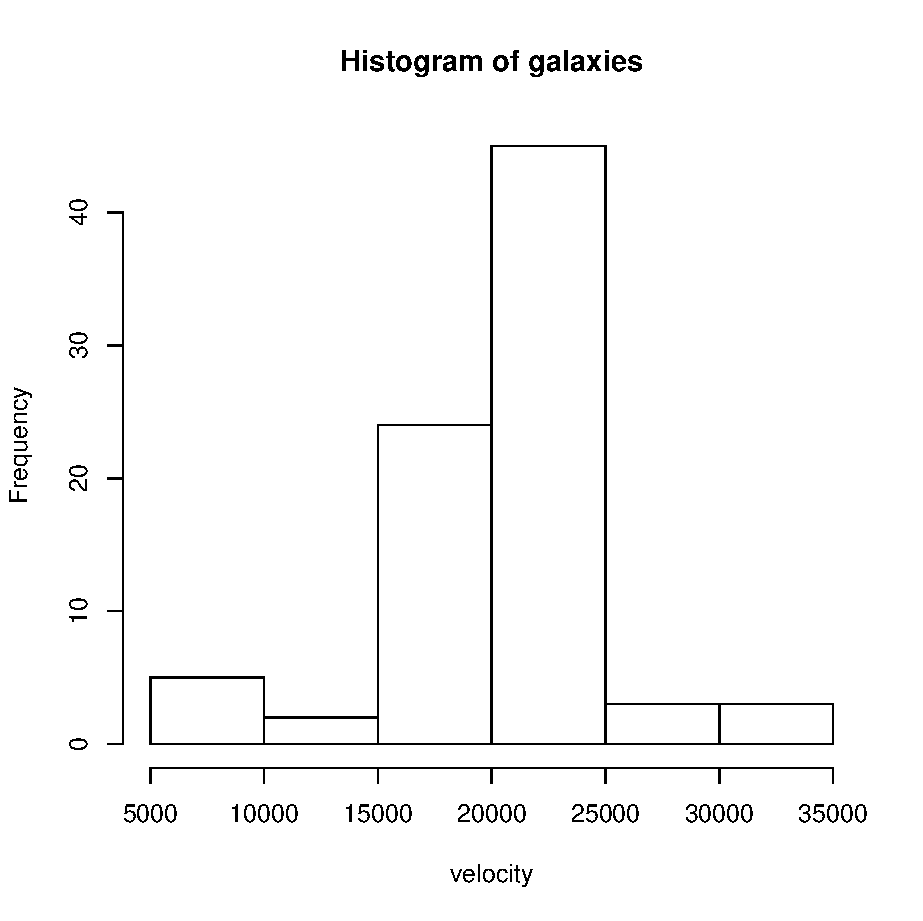
\includegraphics[width=3.0in]{pbdDEMO-include/pics/galaxy_1}
  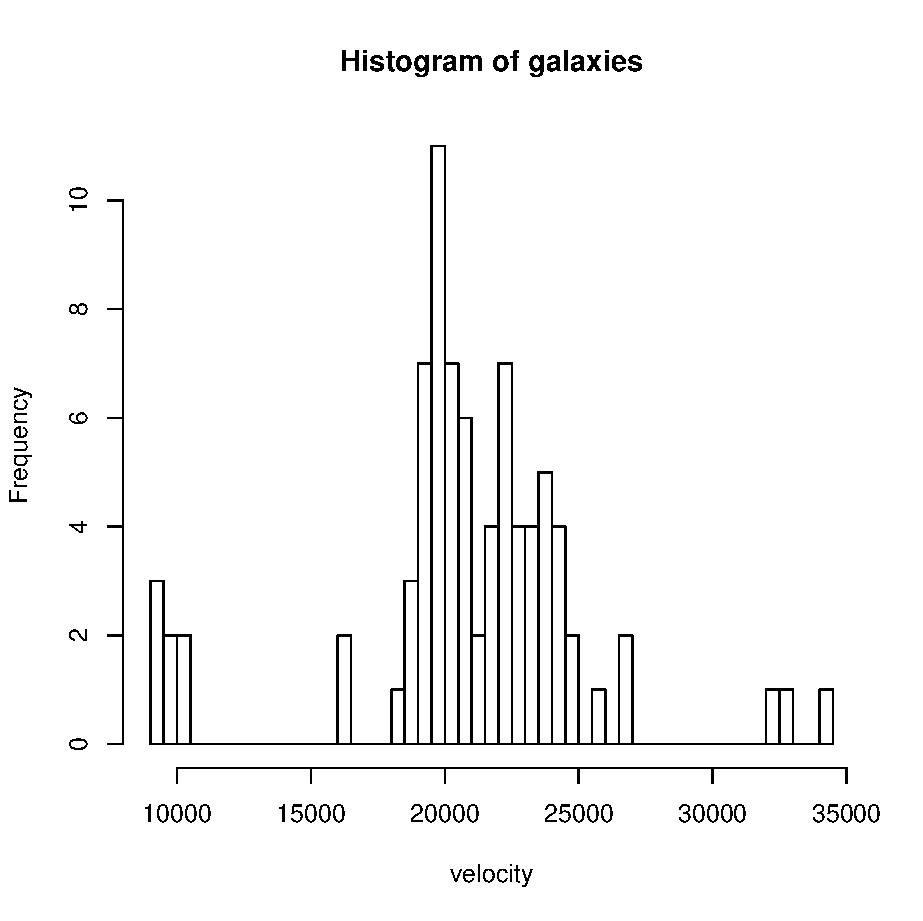
\includegraphics[width=3.0in]{pbdDEMO-include/pics/galaxy_2}
\caption[Histograms of velocities of 82 galaxies]{The left plot is based on
default setting of \code{hist(galaxies)} and the right plot is based on
\code{hist(galaxies, nclass=50)} providing more details of distribution.}
\label{fig:galaxy}
\end{figure}

Suppose we are interesting in the mean velocity of those galaxies and want to
model them as Equations~(\ref{eqn:normal_prior}), (\ref{eqn:normal_likelihood}),
and (\ref{eqn:normal_posterior}).
An example code is given in the \pkg{pbdDEMO} demo via
\begin{lstlisting}
### At the shell prompt, run the demo with 4 processors by
### (Use Rscript.exe for windows system)
mpiexec -np 4 Rscript -e "demo(mcmc_galaxy,'pbdDEMO',ask=F,echo=F)"
\end{lstlisting}
The example has outputs next that it updates 11000 iterations
in total, collects samples in every 10 iterations after 1000 burnin iterations,
and 1000 samples totally collected for inference. The posterior mean of
$\mu$ (velocity of those galaxies) is about $20,820.92$ km/sec and
$95\%$ credible interval is $(19816.91, 21851.07)$ km/sec.
\begin{CodeOutput}
Total iterations: 11000
Burnin: 1000
Thinning: 10
Total samples: 1000
Posterior mean: 20820.92
95% credible interval:
    2.5%    97.5% 
19816.91 21851.07 
\end{CodeOutput}
Also, Figure~\ref{fig:mcmc_galaxy} provides the MCMC trace and
posterior distribution of $\mu$ based on those 1000 samples.
\begin{figure}[ht]
\centering
  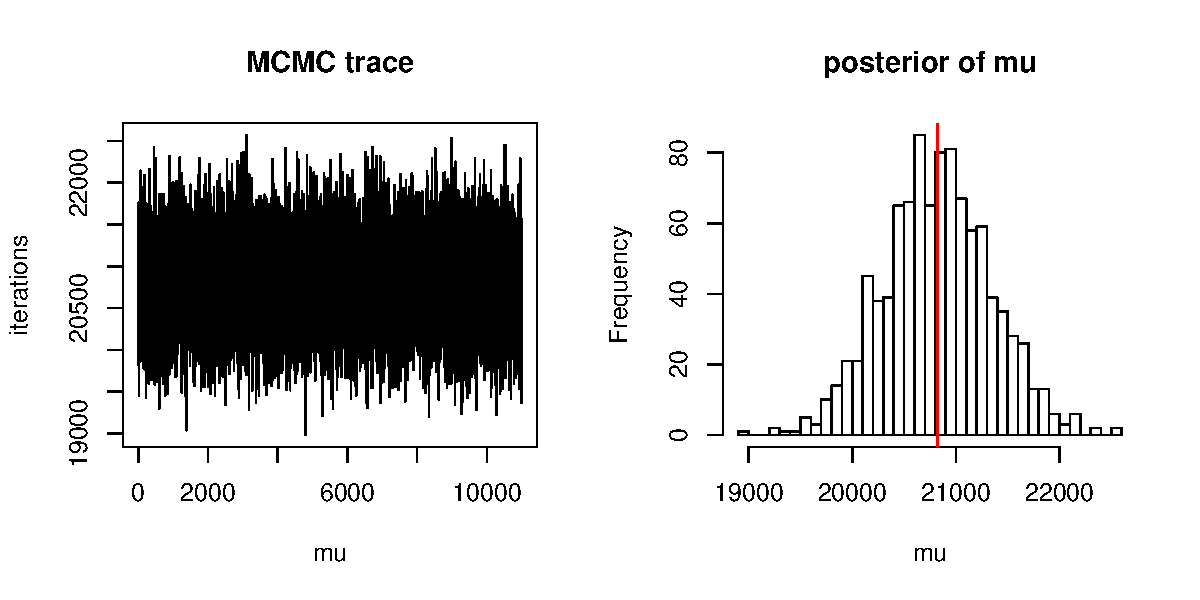
\includegraphics[width=6.0in]{pbdDEMO-include/pics/galaxy_mcmc}
\caption[MCMC results of velocities of 82 galaxies]{
The left plot shows the MCMC trace of 11,000 iterations.
The right plot displays the posterior distribution of $\mu$ in 1000 samples
and red line indicates the posterior mean.}
\label{fig:mcmc_galaxy}
\end{figure}


\section{Parallel Random Number Generator}
\label{sec:prng}
\index{RNG!Parallel Random Number Generator}

We demonstrate a simple MCMC example to fit a
Gaussian model to Galaxy dataset in Section~\ref{sec:galaxy}, but
intend to raise an important issue ``parallel random number generator''
to simulation technique especially in distributed environment.
Even there is no need to use parallel random number generator, but the
purpose here is to explain when to synchronize the random number
if models are getting more complex.

\pkg{pbdMPI} builds in parallel random number generator via
\pkg{rlecuyer}~\citep{rlecuyer}~\index{Package!\pkg{rlecuyer}},
and \code{comm.set.seed(..., diff = TRUE)} is setting different
streams of random numbers to all processors. Suppose different streams
provide independent (or closely) random variables, then every processor
can perform MCMC on local data independently. However,
new parameters and the decision for the new parameters,
should be consistent in all processors so that synchronization is necessary
in some stages of each MCMC iteration.

The Galaxy demo code uses 4 processors to
hold the dataset and every processor start from the different seed to generate
new $\mu$ and uniform random variable $U$ for rejection ratio, but only the
values on rank 0 are \code{bcast()} and used by all other ranks.
\begin{lstlisting}[language=rr,title=Hastings-Metropolis MCMC]
ret <- NULL
ret.all <- NULL
mu.org <- rnorm(1, mean = mu.0, sd = sigma.0)
# No need to synchronize if diff = FALSE in comm.set.seed().
mu.org <- bcast(mu.org)
for(i in 1:(I.b + I.t * I.n)){
  mu.new <- rnorm(1, mean = mu.0, sd = sigma.0)
  # No need to synchronize if diff = FALSE in comm.set.seed().
  mu.new <- bcast(mu.new)

  a <- acceptance(x.gbd, mu.new, mu.org)
  U <- runif(1)
  # No need to synchronize if diff = FALSE in comm.set.seed().
  U <- bcast(U)

  if(U <= a){
    mu.org <- mu.new
  }

  ret.all <- c(ret.all, mu.org)
  if(i > I.b && (i %% I.t == 0)){
    ret <- c(ret, mu.org)
  }
}
\end{lstlisting}
Although we can use \code{comm.set.seed(..., diff = FALSE)} as default,
the parameter $\mu$ and $U$ are tiny and in common of all ranks so that
the cost of communication is relative small. For more complex models,
we may consider to distribute parameters as well and make decision locally,
then we can reduce the cost further. In such cases, parallel random
number generators are better solutions.



\section{Exercises}
\label{sec:bayes_exercise}

\begin{enumerate}[label=\thechapter-\arabic*]

\item
Prove Equation~(\ref{eqn:normal_posterior}) and claim it is conjugate.
{\color{blue} Hint: Equation~(\ref{eqn:propto}). }

\item
Prove Equation~(\ref{eqn:normal_prediction}) and explain intuitively why
the variance of predictive sample is increased comparing with that of
observed samples.
{\color{blue} Hint: is a 95\% predictive interval wider than a 95\% confidence
interval. }

\item
Claim that Equation~(\ref{eqn:acceptant_probability}) is the solution of
Equation~(\ref{eqn:acceptant_rejection}).
{\color{blue} Hint: when is $a(\theta^{(i)} | \theta) = 1$? }

\item
Prove the proposal distribution $q$ with
Equation~(\ref{eqn:acceptant_probability}) provides the desired
distribution $p$.
{\color{blue} Hint: Acceptance-Rejection Sampling algorithm. }

\item
Claim that the upper bound of Equation~(\ref{eqn:accpetance}) controls
the performance of Hastings-Metropolis algorithm.
{\color{blue} Hint: what if
$q(\theta | \theta^{(i)}) \equiv p(\theta | \theta^{(i)})$? }

\item
Discuss when Hastings-Metropolis algorithm fails. Provide an example
that is an inefficient case of Hastings-Metropolis algorithm.
{\color{blue} Hint: What are requirements of Markov Chain? }

\item
Extend the model and algorithm of galaxy velocities example
for unknown mean and unknown variance. e.g.
\begin{eqnarray*}
\bx & \stackrel{i.i.d.}{\sim} & N(\mu, \sigma^2) \\
\mu & \sim & N(\mu_0, \sigma_0^2) \\
\sigma & \sim & Gamma(\alpha_0, \beta_0)
\end{eqnarray*}
Find the 95\% creditable region for $(\mu|\bx, \sigma|\bx)$.

\item
Section~\ref{sec:galaxy} only considers homogeneous distribution for all
galaxy velocities. As model-based clustering in Section~\ref{chp:pmclust},
please extend to a two clusters problem and implement it in Bayesian
framework.

\item
At the end of Section~\ref{sec:prng}, we mention a potential case to avoid
communication for generating new parameters of complex MCMC models.
Given an example and implement in two different ways, one uses parallel
random numbers and the other uses traditional random numbers plus
synchronization.

\end{enumerate}

